

%%%%%%%%%%%%%%%%%%%%% LateX template %%%%%%%%%%%%%%%%%


%%%%%%%%%%%% inicio del documento incluyendo opciones %%%%%%%%%%%%%%%%%%%%%%%%%%%%%%%
\documentclass[letterpaper,11pt]{article}
%%%%%%%%%%%%%%%%%%%%%%%%%%%%%%%%%%%%%%%%%%%%%%%%%%%%%%%%%%%%%%%%%%%%%%%%%%%%

%%%%%%% paquetes utiles: español, incluir graficos, etc %%%%%%%%%%%%%%%%%%%%%%%%%%%%
\usepackage[utf8]{inputenc}
\usepackage{amsmath}
\usepackage{amsfonts}
\usepackage{amssymb}
\usepackage{amsthm}
\usepackage[spanish]{babel}
\usepackage{latexsym}
\usepackage{euscript}
\usepackage{graphicx}
\usepackage{tdclock}
\usepackage{braket}
\usepackage[autostyle=true]{csquotes}
\usepackage{braket}
\usepackage{pdfpages}
\usepackage{subcaption}
\usepackage{hyperref}
%%%%%%%%%%%%%%%%%%%%%%%%%%%%%%%%%%%%%%%%%%%%%%%%%%%%%%%%%%%%%%%%%%%%%%%%%%%%%%%%%%

%%%%%%%%%%%%%%%%%%% espacio para la primera linea del parrafo %%%%%%%%%%%%%%%
\setlength{\parindent}{0mm} 
%%%%%%%%%%%%%%%%%%%%%%%%%%%%%%%%%%%%%%%%%%%%%%%%%%%%%%%%%%%%%%%%%%%%%%%%%%

%%%%%%%%%%%%%%% espacio entre parrafos %%%%%%%%%%%%%%%%%%%%%%%%%%%%%%%
\setlength{\parskip}{2mm}
%%%%%%%%%%%%%%%%%%%%%%%%%%%%%%%%%%%%%%%%%%%%%%%%%%%%%%%%%%%%%%%%%%%%

%%%%%%%%%%%%%%%%%%%%% espaciado entre lineas %%%%%%%%%%%%%%%%%%%%%%%%%%%%%
\linespread{1} 
%%%%%%%%%%%%%%%%%%%%%%%%%%%%%%%%%%%%%%%%%%%%%%%%%%%%%%%%%%%%%%%%%%%%%%

\renewcommand{\vec}[1]{\mathbf{#1}}

%%%%%%%%%%%%%%%%%%%%%%%% Control de margenes %%%%%%%%%%%%%%%%%%%%%%%%%%%%
%\setlength{\topmargin}{-1.cm}
\setlength{\oddsidemargin}{-.8cm}
\setlength{\evensidemargin}{-.8cm}
\setlength{\textheight}{24cm} 
\setlength{\textwidth}{18cm} 
\setlength{\headsep}{-2cm}
%%%%%%%%%%%%%%%%%%%%%%%%%%%%%%%%%%%%%%%%%%%%%%%%%%%%%%%%%%%%%%%%%%%%%%%%%%%%

%%%%%%%%%%%%%%%  definicion de comandos que se utilicen frecuentemente %%%%%%%%%%%%%%%
\def\und#1{\underline{#1}}
\def\be{\begin{equation}}
\def\ee{\end{equation}}
\def\bea{\begin{eqnarray}}
\def\eea{\end{eqnarray}}
%%%%%%%%%%%%%%%%%%%%%%%%%%%%%%%%%%%%%%%%%%%%%%%%%%%%%%%%%%%%%%%%%%%%%%%%%%%%%%%%%%%%

%%%%%%%%%%% Aqui se inicia el contenido del documento %%%%%%%%%%%%%%%%%%%%%%%%%%%%%%%%
\begin{document}

\begin{center}
{\bf \Large Evolución temporal de paquete gaussiano} 
\end{center}

\noindent
{\bf \large Carlos Manuel Rodríguez Martínez} \hspace{5.2cm}

\smallskip


\section{Método numérico}
A continuación se muestra un método numérico para calcular la evolución temporal de un paquete gaussiano. El código en Mathematica es una reimplementación del que se muestra en \url{http://jakevdp.github.io/blog/2012/09/05/quantum-python/}.

Para obtener la evolución temporal del paquete gaussiano se utilizará un método numérico. Partiendo de la ecuación de Schrödinger,
\[
	i \hbar \frac{\partial \psi}{\partial t} = - \frac{\hbar^2}{2 m} \frac{\partial^2 \psi}{\partial x^2} + V \psi.
\]
con la transformada de Fourier
\[
	\tilde{\psi} (k,t) = \frac{1}{\sqrt{2 \pi}} \int_{-\infty}^\infty \psi(x,t) e^{i k x} \, dx,
\]
se llega a la representación de la ecuación de Scrödinger en el espacio de Fourier
\[
	i \hbar \frac{\partial \tilde{\psi}}{\partial t} = \frac{\hbar^2 k^2}{2m} \tilde{\psi} + V \left( i \frac{\partial}{\partial k} \right) \tilde{\psi}.
\]
La aproximación consiste en resolver ambas ecuaciones para intervalos temporales pequeños sin considerar los términos que depende de la derivada de $x$ y $k$. Entonces queda
\[
	i \hbar \frac{\partial \psi}{\partial t} = V(x) \psi
\]
cuya solución es
\[
	\psi(x, t + \Delta t) = \psi(x,t) e^{- \frac{i V(x) \Delta t}{\hbar}},
\]
y de la ecuación de Scrödinger en el espacio de Fourier
\[
	i \hbar \frac{\partial \tilde{\psi}}{\partial t} = \frac{\hbar^2 k^2}{2 m} \tilde{\psi},
\]
cuya solución es
\[
	\tilde{\psi}(k, t+\Delta t) = \tilde{\psi}(k, t) e^{- \frac{i \hbar k^2 \Delta t}{2 m}}.
\]

Para resolver el problema numéricamente conviene discretizarlo, de manera que se usará una transformada de Fourier discreta,
\[
	\widetilde{F_m} = \sum_{n=0}^{N-1} F_n e^{-2\pi i n m / N},
\]
y su inversa
\[
	F_n = \frac{1}{N} \sum_{m=0}^{N-1} \widetilde{F_m} e^{2\pi i n m / N}.
\]
Para llegar a esta forma discreta primero se hará la consideración de que el potencial tiende a infinito para los valores $x \le a$ y $x \ge b$. Entonces
\[
	\widetilde{\psi}(k, t) = \frac{1}{\sqrt{2\pi}}
   \int_a^b \psi(x, t) e^{-ikx} dx.
\]
Al aproximar la integral por una suma de Riemman de $N$ términos, con $\Delta x = (b - a) / N$ y $x_n = a + n\Delta x$ queda
\[
	\widetilde{\psi}(k, t) \simeq \frac{1}{\sqrt{2\pi}}
   \sum_{n=0}^{N-1} \psi(x_n, t) e^{-ikx_n} \Delta x.
\]
Por último se hace $k_m = k_0 + m\Delta k$, con $\Delta k = 2\pi / (N\Delta x)$, y queda
\[
	\widetilde{\psi}(k_m, t) \simeq \frac{1}{\sqrt{2\pi}}
   \sum_{n=0}^{N-1} \psi(x_n, t) e^{-ik_m x_n} \Delta x.
\]
Sustituyendo esto en la expresión para la transformada de Fourier discreta se llega a
\[
	\left[\widetilde{\psi}(k_m, t) e^{i m x_0 \Delta k}\right]
   \simeq \sum_{n=0}^{N-1} 
   \left[ \frac{\Delta x}{\sqrt{2\pi}}
   \psi(x_n, t) e^{-ik_0 x_n} \right]
   e^{-2\pi i m n / N}
\]
y para la transformada de Fourier inversa
\[
	\left[\frac{\Delta x}{\sqrt{2 \pi}} \psi(x_n, t) e^{-i k_0 x_n}\right]
   \simeq \frac{1}{N} \sum_{m=0}^{N-1} 
   \left[\widetilde{\psi}(k_m, t) e^{-i m x_0 \Delta k} \right]
   e^{2\pi i m n / N}.
\]
Este resultado nos indica que el par
\[
	\psi(x, t) \Longleftrightarrow \widetilde{\psi}(k, t)
\]
en el caso continuo corresponde al par
\[
   \frac{\Delta x}{\sqrt{2 \pi}} \psi(x_n, t) e^{-i k_0 x_n}
   \Longleftrightarrow
   \widetilde{\psi}(k_m, t) e^{-i m x_0 \Delta k}
\]
en el caso discreto con las aproximaciones. Con esto se puede construir un algoritmo para evaluar la evolución temporal de la función de onda.

\begin{enumerate}
\item Se escogen $a$, $b$, $N$ y $k_0$ suficientes para representar el estado inicial de la función de onda $\psi(x)$. Con esto se puede calcular $\Delta x = (b - a) / N$ y $\Delta k = 2\pi / (b - a)$.  Se definen también los arrays
   $x_n = a + n \Delta x$ y $k_m = k_0 + m \Delta k$.
   
\item Se discretiza la función de onda en el array. Sea $\psi_n(t) = \psi(x_n, t)$, $V_n = V(x_n)$, y $\widetilde{\psi}_m = \widetilde{\psi}(k_m, t)$.

\item Para avanzar el sistema en intervalo temporal $\Delta t$ se hace lo siguiente.
Se computa un medio paso en $x$,
\[
\psi_n \longleftarrow \psi_n
       \exp[-i (\Delta t / 2) (V_n / \hbar)]
\]

\item Se calcula $\widetilde{\psi}_m$ de $\psi_n$ usando la transformada de Fourier discreta.

\item Se computa un paso completo en $k$,
\[
	\widetilde{\psi}_m \longleftarrow \widetilde{\psi}_m
      \exp[-i \hbar (k \cdot k) \Delta t / (2 m)].
\]

\item Se calcula $\psi_n$ de $\widetilde{\psi}_m$ usando la transformada de Fourier discreta inversa.

\item Se computa un segundo medio paso en $x$,
\[
\psi_n \longleftarrow \psi_n
       \exp[-i (\Delta t / 2) (V_n / \hbar)]
\]

\item Se repite desde el paso 3 hasta que se avance al tiempo deseado.

\end{enumerate}

El código de Mathematica que implementa este algoritmo es el siguiente
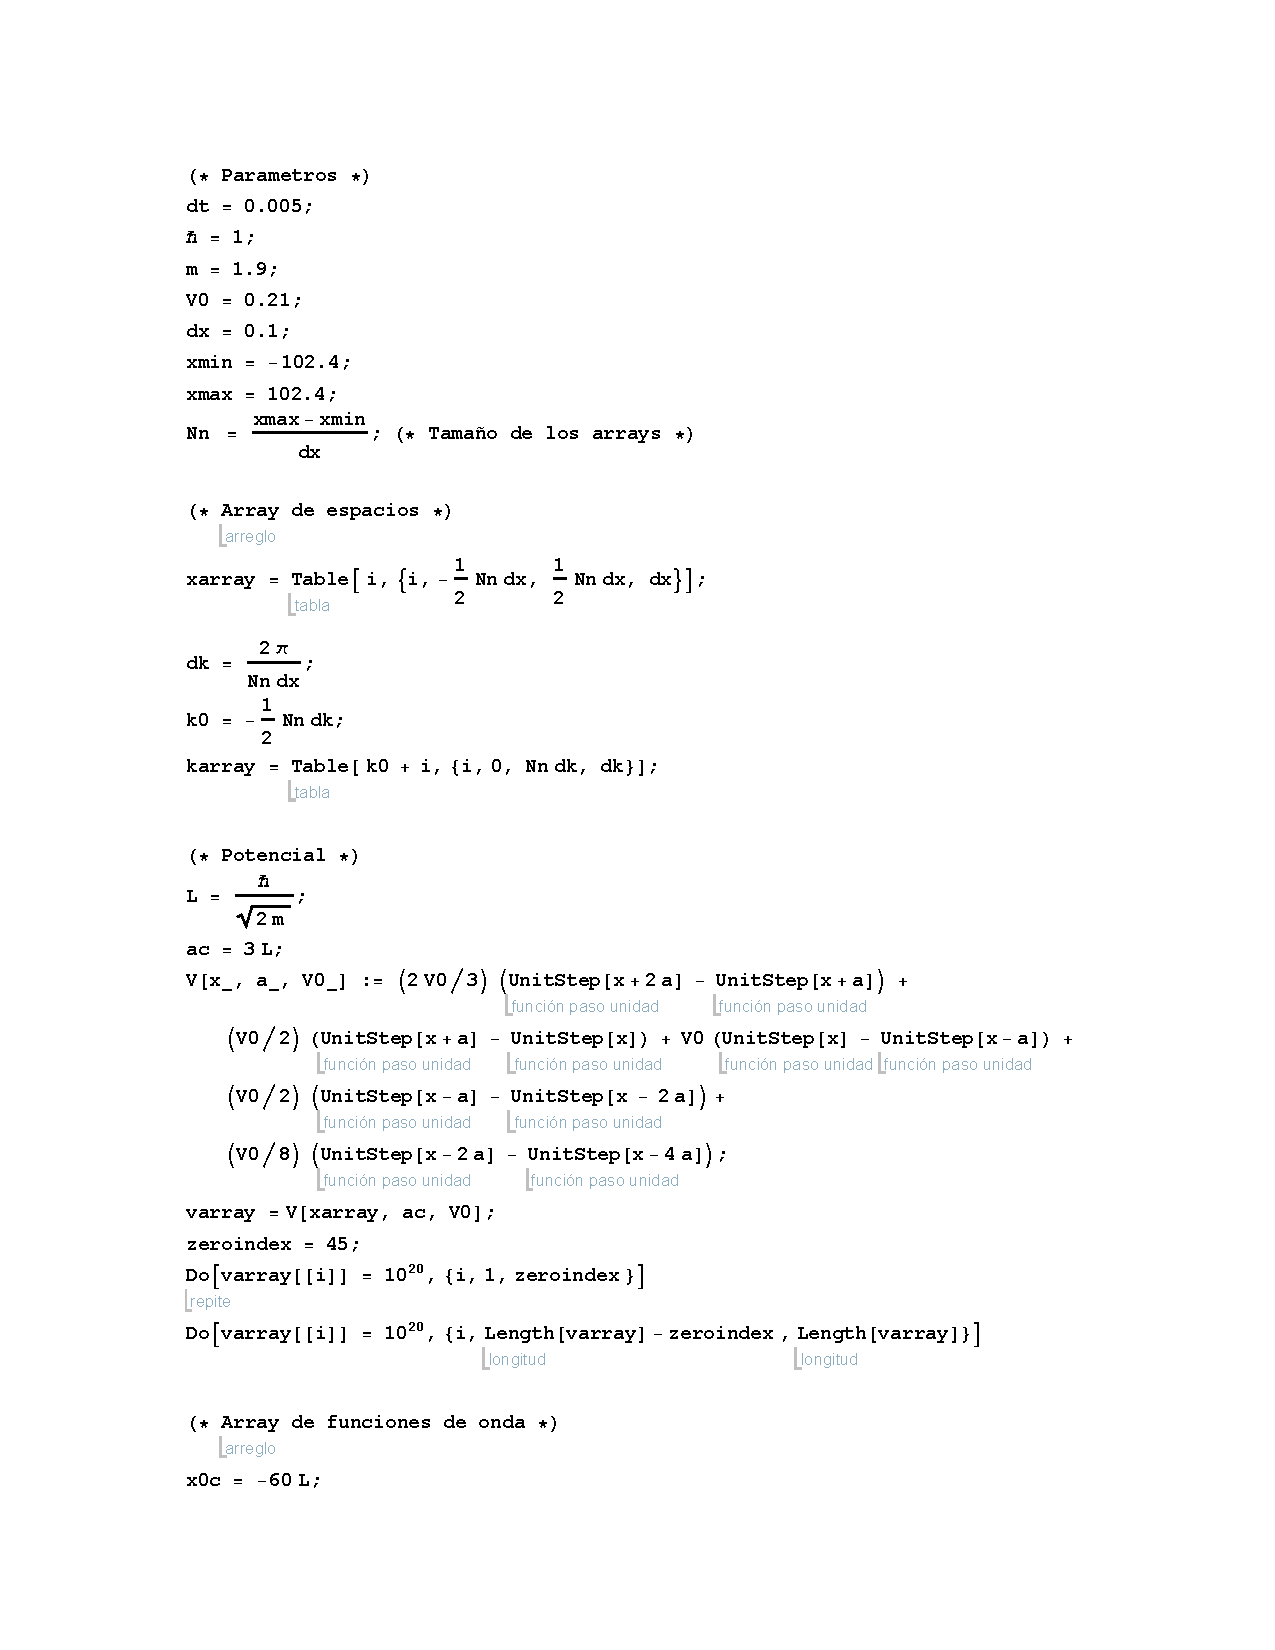
\includepdf[pages=-]{Codigo.pdf}

Las gráficas que se generan son
\begin{figure}[h!]
\begin{subfigure}{.5\textwidth}
	\centering
	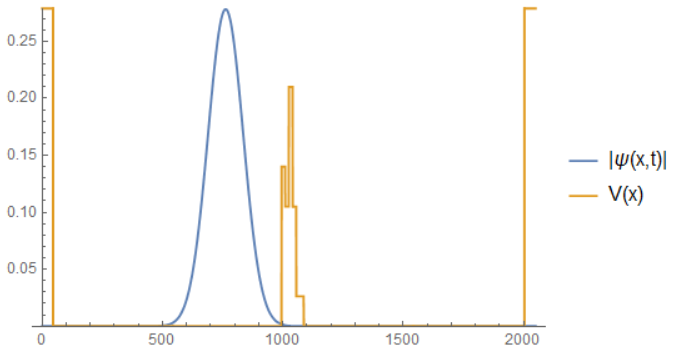
\includegraphics[scale=0.60]{img/grafica1}
	\caption{$t = 10$.}
\end{subfigure}%
\begin{subfigure}{.5\textwidth}
	\centering
	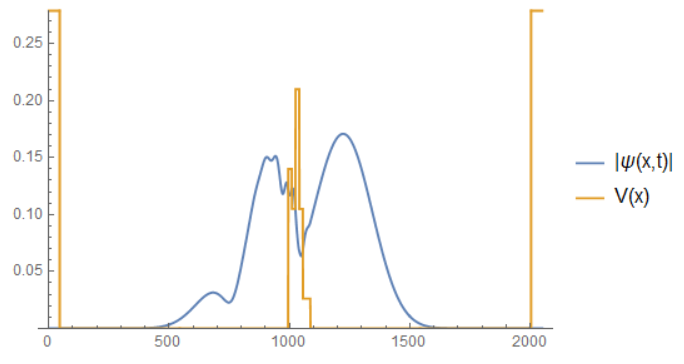
\includegraphics[scale=0.60]{img/grafica2}
	\caption{$t=100$.}
\end{subfigure}%
\caption{Gráficas de la evolución temporal.}
\end{figure}

\end{document}
